%\documentclass[handout]{beamer}
\documentclass{beamer}
\usepackage[utf8]{inputenc}
\usepackage[T1]{fontenc}
\usepackage[swedish,british]{babel}
\usepackage{url}
\usepackage{graphicx}
\usepackage{color}
\usepackage{subfig}
\usepackage{multicol}
\usepackage{amssymb,amsmath,amsthm}
\usepackage{booktabs}
\usepackage[squaren,binary]{SIunits}
\usepackage[strict]{csquotes}
\usepackage{cleveref}
\usepackage{hhcount}

\setbeamertemplate{bibliography item}[text]
\usepackage[natbib,style=alphabetic,maxbibnames=99]{biblatex}
\addbibresource{basics.bib}

\usepackage{xparse}
\ProvideDocumentEnvironment{exercise}{o}{%
  \setbeamercolor{block body}{bg=yellow!30,fg=black}
  \setbeamercolor{block title}{bg=yellow,fg=black}
  \IfValueTF{#1}{%
    \begin{block}{Exercise: #1}
  }{%
    \begin{block}{Exercise}
  }
}{%
  \end{block}
}

\DeclareMathOperator{\powerset}{\mathcal{P}}
\DeclareMathOperator{\p}{\mathcal{P}}
\let\P\p
\DeclareMathOperator{\C}{\mathcal{C}}
\DeclareMathOperator{\K}{\mathcal{K}}
\DeclareMathOperator{\E}{\mathcal{E}}
\DeclareMathOperator{\D}{\mathcal{D}}

\DeclareMathOperator{\N}{\mathbb{N}}
\DeclareMathOperator{\Z}{\mathbb{Z}}
\DeclareMathOperator{\R}{\mathbb{R}}

\let\stoch\mathbf{}

\DeclareMathOperator{\xor}{\oplus}

\renewcommand{\qedsymbol}{Q.E.D.}

\mode<presentation>{%
  \usetheme{Berlin}
  \setbeamercovered{transparent}
}
\setbeamertemplate{footline}{\insertframenumber}

\title{%
  Elementary Information Theory
}
\author{%
  Daniel Bosk
}
\institute[MIUN IKS]{%
  Department of Information and Communication Systems,\\
  Mid Sweden University, Sundsvall.
}
\date{\today}

\AtBeginSection[]{%
  \begin{frame}
    \tableofcontents[currentsection]
  \end{frame}
}

\begin{document}

\begin{frame}
  \titlepage{}
\end{frame}

\begin{frame}
  \tableofcontents
\end{frame}


% Since this a solution template for a generic talk, very little can
% be said about how it should be structured. However, the talk length
% of between 15min and 45min and the theme suggest that you stick to
% the following rules:  

% - Exactly two or three sections (other than the summary).
% - At *most* three subsections per section.
% - Talk about 30s to 2min per frame. So there should be between about
%   15 and 30 frames, all told.


\section{Introduction}

\subsection{History}

\begin{frame}
  \begin{itemize}
    \item Created 1948 by Shannon's paper 
      \citetitle{Shannon1948amt}~\cite{Shannon1948amt}.

      \pause{}

    \item He starts using the term \enquote{entropy} as a measure for 
      information.
      \begin{itemize}
        \item In physics entropy measures the disorder of molecules.
        \item Shannon's entropy measures disorder of information.
      \end{itemize}

      \pause{}

    \item He used this theory to analyse communication.
      \begin{itemize}
        \item What are the theoretical limits for different channels?
        \item How much redundancy is needed for certain noise?
      \end{itemize}

  \end{itemize}
\end{frame}

\begin{frame}
  \begin{itemize}
    \item This theory is interesting on the physical layer of networking.

      \pause{}

    \item It's also interesting for security.
      \begin{itemize}
        \item Field of Information Theoretic Security
        \item \enquote{Efficiency} of passwords
        \item Measure identifiability
        \item \dots
      \end{itemize}
  \end{itemize}
\end{frame}

\begin{frame}
  \begin{itemize}
    \item Information Theory is based in Probability Theory.
    \item So we need a slight recap.
  \end{itemize}
\end{frame}


\section{Probability theory}

\subsection{Some definitions}

\begin{frame}
  \begin{definition}[Outcome]
    \begin{itemize}
      \item \emph{Sample space} \(\Omega\) of all possible outcomes.
      \item Elements \(\omega\in \Omega\) are called outcomes.
      \item An \emph{event} is a set \(A\subseteq \Omega\).
    \end{itemize}
  \end{definition}
\end{frame}

\begin{frame}
  \begin{example}
    \begin{itemize}
      \item Sample space of a roll of a die: \[\Omega_D = \{\fcdice{1}, 
          \fcdice{2}, \fcdice{3}, \fcdice{4}, \fcdice{5}, \fcdice{6}\},\]
        
        \pause{}

      \item The set of possible events is \(\powerset(\Omega_D) 
          = \{\{\fcdice{1}\}, \ldots, \{\fcdice{6}\}, \{\fcdice{1}, 
          \fcdice{2}\}, \ldots, \{\fcdice{1}, \fcdice{6}\}, 
          \{\fcdice{2},\fcdice{3}\}, \ldots, 
          \{\fcdice{1},\ldots,\fcdice{6}\}\}\).
      \item Thus \(\{\fcdice{1}\},\ldots,\{\fcdice{6}\}\) are events.
      \item But so is \(\emptyset\) and \(\{\fcdice{1}, \ldots, \fcdice{6}\}\).

        \pause{}

      \item An event means that one of its outcomes happen.
      \item So that we can express \enquote{the die roll results in an even 
          number}: \(\{\fcdice{2}, \fcdice{4}, \fcdice{6}\}\).
    \end{itemize}
  \end{example}
\end{frame}

\begin{frame}
  \begin{definition}[Probability measure]
    \begin{itemize}
      \item \(\Omega\) is a sample space.
      \item A \emph{probability measure} is a function \(\Pr\colon 
          \powerset(\Omega)\to [0,1]\) such that:
        \begin{enumerate}
          \item \(\Pr[ \emptyset ] = 0\) and \(\Pr[ \Omega ] = 1\),
          \item If \(A\subseteq \Omega\) and \(B\subseteq \Omega\) and \(A\cap 
              B = \emptyset\), then \(\Pr[A\cup B] = \Pr[A] + \Pr[B]\).
        \end{enumerate}
    \end{itemize}
  \end{definition}

  \begin{exercise}
    This is well-defined, but why?
    For instance, how do we know that \(0\leq \Pr[A] + \Pr[B]\leq 1\)?
  \end{exercise}
\end{frame}

\begin{frame}
  \begin{example}
    \begin{itemize}
      \item Let \(\Omega_D\) be the sample space for the die roll.
      \item How shall we define \(\Pr\colon \powerset(\Omega_D)\to [0, 1]\)?

        \pause{}

      \item \(\Pr[\{\fcdice{1}\}] = \cdots = \Pr[\{\fcdice{6}\}] 
          = \frac{1}{6}\)
    \end{itemize}
  \end{example}

  \pause{}

  \begin{exercise}
    The probability of the die showing an even number after a roll is 
    \(\frac{3}{6}\), why?
  \end{exercise}
\end{frame}

\begin{frame}
  \begin{definition}[Probability space]
    \begin{itemize}
      \item \(\Omega\) is a sample space.
      \item \(\Pr\) is a probability measure on \(\Omega\).

        \pause{}

      \item We call \((\Omega, \Pr)\) for a \emph{probability space}.
    \end{itemize}
  \end{definition}
\end{frame}

\subsection{Some results}

\begin{frame}
  \begin{theorem}[Probability for event and complement]
    \begin{itemize}
      \item Let \(A\subseteq \Omega\) be an event and \(C = \Omega\setminus A\) 
        its complement.
      \item Then \(\Pr[C] = 1 - \Pr[A]\).
    \end{itemize}
  \end{theorem}

  \pause{}

  \begin{proof}
    \begin{itemize}
      \item Definition said \(\Pr[\Omega] = 1\).

        \pause{}

      \item \(A\cup C = \Omega\), thus \(\Pr[A\cup C] = 1\).

        \pause{}

      \item It also said that for \(A\subseteq \Omega\) and \(B\subseteq 
          \Omega\) we have \(\Pr[A\cup B] = \Pr[A] + \Pr[B]\).

        \pause{}

      \item So \(\Pr[A\cup C]\) is also \(\Pr[A] + \Pr[C]\).

        \pause{}

      \item Thus \(\Pr[A] + \Pr[C] = 1\) and so \(\Pr[C] = 1 - \Pr[A]\).
    \end{itemize}
  \end{proof}
\end{frame}

\begin{frame}
  \begin{example}
    \begin{itemize}
      \item Rolling an even number was probability \(\frac{3}{6}\).
      \item Applying the theorem, rolling an odd number is \(1-\frac{3}{6}\).
    \end{itemize}
  \end{example}

  \pause{}

  \begin{exercise}
    Give two ways to compute the probability of rolling a \fcdice{6}.
  \end{exercise}
\end{frame}

\begin{frame}
  \begin{definition}[Independent evens]
    \begin{itemize}
      \item \((\Omega, \Pr)\) is a probability space.
      \item Events \(A\subseteq \Omega\) and \(B\subseteq \Omega\) are 
        \emph{independent} if \(\Pr[A\cap B] = \Pr[A]\cdot \Pr[B]\).
    \end{itemize}
  \end{definition}

  \pause{}

  \begin{example}
    \begin{itemize}
      \item We roll one die, \(\Omega_D = \{\fcdice{1}, \ldots, \fcdice{6}\}\).
      \item Events: roll a one, \(A = \{\fcdice{1}\}\), and roll a six, \(B 
          = \{\fcdice{6}\}\).

        \pause{}

      \item Clearly we cannot get \fcdice{1} and \fcdice{6} at the same time:
        \[\Pr[A\cap B] = \Pr[\emptyset] = 0 \neq \Pr[A]\cdot \Pr[B].\]

      \item But we can get either: \(\Pr[A\cup B] = \Pr[A] + \Pr[B] 
          = \frac{2}{6}\).
    \end{itemize}
  \end{example}
\end{frame}

\begin{frame}
  \begin{example}
    \begin{itemize}
      \item We roll two dice: \(\Omega_{D2} = \{(\fcdice{1},\fcdice{1}), 
          \ldots, (\fcdice{1}, \fcdice{6}), \ldots, (\fcdice{6}, \fcdice{1}), 
          \ldots, (\fcdice{6}, \fcdice{6})\).

        \pause{}

      \item Roll a one: \(A = \{(\fcdice{1}, \fcdice{1}), \ldots, (\fcdice{1}, 
          \fcdice{6}), (\fcdice{2}, \fcdice{1}), \ldots, (\fcdice{6}, 
          \fcdice{1})\}\).

      \item Roll a six: \(B = \{(\fcdice{6}, \fcdice{1}), \ldots, (\fcdice{6}, 
          \fcdice{6}), (\fcdice{1}, \fcdice{6}), \ldots, (\fcdice{5}, 
          \fcdice{6})\}\).

        \pause{}

      \item Roll a one and a six: \(\Pr[A\cap B] = \Pr[\{(\fcdice{1}, 
          \fcdice{6}), (\fcdice{6}, \fcdice{1})\}] = \frac{2}{36} \neq 
          \frac{1}{6}\cdot \frac{1}{6}\).

      \item Roll a one or a six with two chances: \(\Pr[A\cup B]\).

    \end{itemize}
  \end{example}
\end{frame}

\begin{frame}
  \begin{example}
    \begin{itemize}
      \item We roll two dice: \(\Omega_{D2} = \{(\fcdice{1},\fcdice{1}), 
          \ldots, (\fcdice{1}, \fcdice{6}), \ldots, (\fcdice{6}, \fcdice{1}), 
          \ldots, (\fcdice{6}, \fcdice{6})\).

        \pause{}

      \item \emph{First} roll a one: \(A = \{(\fcdice{1}, \fcdice{1}), \ldots, 
          (\fcdice{1}, \fcdice{6})\}\).

      \item \emph{Second} roll a six: \(B = \{(\fcdice{1}, \fcdice{6}), \ldots, 
          (\fcdice{6}, \fcdice{6})\}\).

        \pause{}

      \item First roll a one, then a six: \(\Pr[A\cap B] = \Pr[\{(\fcdice{1}, 
          \fcdice{6})\}] = \frac{1}{36} = \frac{1}{6}\cdot \frac{1}{6}\).

      \item Either roll a one first \emph{or} a six on the second: \(\Pr[A\cup 
          B]\).

    \end{itemize}
  \end{example}
\end{frame}

\begin{frame}
  \begin{exercise}
    Even if \(\Pr[A]\cdot \Pr[B] = \Pr[A\cap B]\) they are not necessarily 
    independent, why?
  \end{exercise}
\end{frame}

\subsection{Conditional probability}

\begin{frame}
  \begin{definition}[Conditioned probability]
    \begin{itemize}
      \item Let \(A, B\) be events in probability space \((\Omega, \Pr)\).
      \item The probability of \(B\) given \(A\) is defined as \(\Pr[B\mid A] 
          = \frac{\Pr[B\cap A]}{\Pr[A]}\)
    \end{itemize}
  \end{definition}

  \pause{}
  
  \begin{example}
    \begin{itemize}
      \item Use probability space for rolling a die, \((\Omega_D, \Pr)\).
      \item Event \(E = \{\fcdice{2}, \fcdice{4}, \fcdice{6}\}\) for even side 
        up.

        \pause{}

      \item Let \(A = \{\fcdice{2}\}\) and \(B = \{\fcdice{3}\}\), then
        \[\Pr[A\mid E] = \frac{\Pr[\{\fcdice{2}\}]}{\Pr[E]} = \frac{1}{3}
          \text{ and }
          \Pr[B\mid E] = \frac{\Pr[\emptyset]}{\Pr[E]} = 0.\]

    \end{itemize}
  \end{example}
\end{frame}

\begin{frame}
  \begin{theorem}[Joint probability]
    \begin{itemize}
      \item Let \(A, B\) be events in probability space \((\Omega, \Pr)\).
      \item Then \(\Pr[A\cap B] = \Pr[A]\cdot \Pr[B\mid A]\)
    \end{itemize}
  \end{theorem}

  \pause{}

  \begin{exercise}
    Using conditional probability we can show this new result, how?
  \end{exercise}
%  \begin{proof}
%    \begin{itemize}
%      \item We know from definition: \(\Pr[B\mid A] = \frac{\Pr[A\cap 
%            B]}{\Pr[A]}\).
%
%      \item Thus \(\Pr[B\mid A]\cdot \Pr[A] = \Pr[A\cap B]\).
%    \end{itemize}
%  \end{proof}
\end{frame}

\begin{frame}
  \begin{theorem}[Bayes sats]
    \begin{itemize}
      \item Let \(A, B\) be events in probability space \((\Omega, \Pr)\).
      \item Then \(
          \Pr[A\mid B] = \frac{\Pr[B\mid A]\Pr[A]}{\Pr[B]}.
        \)
    \end{itemize}
  \end{theorem}

  \pause{}

  \begin{proof}
    \begin{itemize}
      \item \(\Pr[A\mid B] = \frac{\Pr[A\cap B]}{\Pr[B]}\) and \(\Pr[B\mid A] 
          = \frac{\Pr[A\cap B]}{\Pr[A]}\).

        \pause{}

      \item Thus \(\Pr[A\cap B] = \Pr[A\mid B] \Pr[B] = \Pr[B\mid A] \Pr[A]\).

        \pause{}

      \item Which means \(\Pr[A\mid B] = \frac{\Pr[B\mid A] \Pr[A]}{\Pr[B]}\).
    \end{itemize}
  \end{proof}
\end{frame}

\begin{frame}
  \begin{example}[An intrusion detection system]
    \begin{itemize}
      \item Our IDS is this good:
        \begin{itemize}
          \item It detects malicious traffic with \unit{99}{\%} certainty (true 
            positives).
          \item It discards benign traffic with \unit{99}{\%} certainty (true 
            negatives).
        \end{itemize}

        \pause{}

      \item \emph{Assume} \unit{0.5}{\%} of \enquote{the traffic} consist of 
        attacks.

        \pause{}

      \item Event \(M\) is malicious traffic, \(B\) is benign traffic.
      \item Event \(+\) means IDS declared malicious, \(-\) declared benign.

        \pause{}

      \item Then we get \dots
    \end{itemize}
  \end{example}
\end{frame}

\begin{frame}
  \begin{example}[IDS continued]
    \begin{align*}
      \Pr[M\mid +] &= \frac{\Pr[+\mid M] \Pr[M]}{\Pr[+]}
      = \frac{0.99\cdot 0.005}{\Pr[+]} \\
      &= \frac{0.99\cdot 0.005}{\Pr[+\mid M] \Pr[M] + \Pr[+\mid B] \Pr[B]} 
      \\
      &= \frac{0.99\cdot 0.005}{0.99\cdot 0.005 + 0.01\cdot (1 - \Pr[M])} 
      \\
      &= \frac{0.99\cdot 0.005}{0.99\cdot 0.005 + 0.01\cdot 0.995} \\
      &= 0.33
    \end{align*}
  \end{example}
\end{frame}

\begin{frame}
  \begin{exercise}
    \begin{itemize}
      \item What's a good-enough probability for \(\Pr[M\mid +]\)?
      \item How do we achieve it?
    \end{itemize}
  \end{exercise}
\end{frame}


\section{Shannon entropy}

\subsection{Definition av Shannonentropi}

\begin{frame}
  \begin{definition}[Shannonentropi]
    Låt \(\stoch X\) vara en stokastisk variabel som antar värden från en 
    ändlig mängd \(X\).
    Då definieras \emph{Shannonentropin} för den stokastiska variabeln 
    \(\stoch X\) som
    \begin{align*}
      H(\stoch X) = -K \sum_{x\in X} \Pr(\stoch X = x)\log \Pr(\stoch X = x),
    \end{align*}
    där \(K\) oftast väljs som \(\frac{1}{\log 2}\).
    Då sägs entropin anges i enheten bitar (\bit).
  \end{definition}
\end{frame}

\begin{frame}
  \begin{itemize}
    \item Vi kan se Shannonentropin för en stokastisk variabel som hur mycket 
      \enquote{val} som varje utfall innebär.

    \item Den kan även tolkas som osäkerheten för ett utfall för variabeln.

    \item Eller hur många bitar som krävs för att lagra resultatet av ett 
      utfall.

    \item Och då naturligtvis ett mått på hur mycket information den 
      producerar.

  \end{itemize}
\end{frame}

\begin{frame}
  \begin{example}[Singla slant]
    Låt \(\stoch S\) beteckna en stokastisk variabel som antar värden ur 
    mängden \(S = \{krona, klave\}\).
    Då har vi att
    \begin{align*}
      \Pr(\stoch S = krona) = p_{krona} = \Pr(\stoch S = klave) &= p_{klave} 
      = \frac{1}{2}.
    \end{align*}
    Entropin för \(\stoch S\) är följaktligen
    \begin{align*}
      H(\stoch S) &= -\left( p_{krona}\log p_{krona} + p_{klave}\log p_{klave} 
      \right) \\
        &= -2\times \frac{1}{2}\log \frac{1}{2} = \log 2 = 1.
    \end{align*}
  \end{example}
\end{frame}

\begin{frame}
  \begin{example}[Kasta tärning]
    Låt \(\stoch T\) beteckna en stokastisk variabel som antar värden ur 
    mängden \(T = \{1, 2, 3, 4, 5, 6\}\).
    Då har vi att \(\Pr(\stoch T = t) = \frac{1}{6}\) för alla \(t\in T\).
    Följaktligen är entropin för \(\stoch T\)
    \begin{align*}
      H(\stoch T) &= -\sum_{t\in T} \Pr(\stoch T = t)\log\Pr(\stoch T = t) \\
      &= -6\times \frac{1}{6}\log\frac{1}{6} = \log 6 \approx 2.585.
    \end{align*}
  \end{example}
\end{frame}

\begin{frame}
  \begin{itemize}
    \item Betyder alltså att det svårare att förutspå ett tärningskast än 
      slantsingling.

    \item För att lagra resultaten av tärningskasten krävs mer utrymme.

    \item Låt oss förvanska tärningen en aning och se vad som händer \dots
  \end{itemize}
\end{frame}

\begin{frame}
  \begin{example}[Tärningskast igen]
    En ny stokastisk variabel \(T^\prime\) antar värden ur \(T = \{1, 2, 3, 4, 
    5, 6\}\).
    Låt nu \(\Pr(\stoch T^\prime = 6) = \frac{9}{10}\) och \(\Pr(\stoch 
    T^\prime = t) = \frac{1}{5\times 10}\) för alla \(t\neq 6\).
    Detta ger entropin
    \begin{align*}
      H(\stoch T^\prime) &= -\left( \frac{9}{10}\log\frac{9}{10} + \sum_{t\neq 
      6} \frac{1}{50}\log\frac{1}{50} \right) \\
        &= -\frac{9}{10}\log\frac{9}{10} -5\times\frac{1}{50}\log\frac{1}{50} 
        \\
        &= -\frac{9}{10}\log\frac{9}{10} -\frac{1}{10}\log\frac{1}{50} \approx 
        0.486.
    \end{align*}
  \end{example}
\end{frame}

\begin{frame}
  \begin{itemize}
    \item Det betyder att det är mycket enklare att förutspå ett kast med denna 
      förvanskade tärning.
    \item Det krävs mindre utrymme att lagra utfallen.
  \end{itemize}
\end{frame}

\subsection{Jensens olikhet}

\begin{frame}
  \begin{definition}
    Låt \(f\colon \R\to \R\) vara en funktion sådan att
    \begin{align*}
      tf(x) + (1-t)f(y) \leq f(tx + (1-t)y),
    \end{align*}
    då säger vi att \(f\) är \emph{konkav}.
    Vid strikt olikhet för \(x\neq y\) säger vi att \(f\) är \emph{strikt 
    konkav}.
  \end{definition}

  \begin{example}
    \(\log\) är en strikt konkav funktion.
  \end{example}
\end{frame}

%\begin{frame}
%  \begin{lemma}
%    Låt \(f\) vara en strikt konkav funktion.
%    Då har vi att
%    \begin{align*}
%      tf(x) + (1-y)f(y) = f( tx + (1-t)y )
%    \end{align*}
%    om och endast om \(x = y\).
%  \end{lemma}
%\end{frame}
%
%\begin{frame}
%  \begin{proof}
%    Antag \(x = y\).
%    Då har vi
%    \begin{align*}
%      tf(x) + (1-t)f(x) = f(x)(t+1-t) = f(x).
%    \end{align*}
%    Men
%    \begin{align*}
%      f(tx + (1-t)x) = f((t+1-t)x) = f(x)
%    \end{align*}
%    och alltså har vi likhet.
%
%    Antag \(tf(x) + (1-t)f(y) = f(tx + (1-t)y)\).
%    Då har vi
%    \begin{align*}
%      t( f(x) - f(y) ) + f(y) = f( t( x - y ) + y ).
%    \end{align*}
%    Högerledet implicerar \(f(x) = f(y)\), men då beror vänterledet enbart på 
%    \(f(y)\) och således måste även \(x = y\).
%  \end{proof}
%\end{frame}

\begin{frame}
  \begin{theorem}[Jensens olikhet]
    Om \(f\) är en strikt konkav funktion och \(a_1, a_2,\ldots, a_n\) är 
    reella tal strikt större än noll och sådana att \(\sum_{i=1}^n a_i = 1\) då 
    gäller att
    \begin{align*}
      \sum_{i=1}^n a_i f(x_i) \leq f\left( \sum_{i=1}^n a_i x_i\right),
    \end{align*}
    med likhet om och endast om \(x_1 = x_2 = \cdots = x_n\).
  \end{theorem}
\end{frame}

%\begin{frame}
%  \begin{block}{Bevis för Jensens olikhet.}
%    Bevis genom induktion.
%    Antag \(n=2\).
%    Då har vi att \(a_1 + a_2 = 1\) och alltså \(a_1 = 1 - a_2\).
%    Eftersom \(f\) är konkav har vi att
%    \begin{align*}
%      a_1f(x_1) + a_2f(x_2) \leq f(a_1x_1 + a_2x_2).
%    \end{align*}
%
%    Antag sant för \(n=k\).
%    \begin{align}
%      \label{eq:JensenIndhyp}
%      \sum_{i=1}^k a_i = 1 \land
%        \sum_{i=1}^k a_if(x_i) \leq f\left( \sum_{i=1}^k a_ix_i\right).
%    \end{align}
%  \end{block}
%\end{frame}
%
%\begin{frame}
%  \begin{proof}[Forts. bevis för Jensens olikhet]
%    Lås oss visa att detta även gäller för \(n=k+1\).
%    Eftersom att \(f\) är konkav gäller att
%    \begin{align}
%      \label{eq:JensenInductive1}
%      \sum_{i=1}^{k+1} a_if(x_i) &= a_1f(x_1) + (1-a_1)\sum_{i=2}^{k+1} 
%      \frac{a_i}{1-a_1}f(x_i) \\
%      \label{eq:JensenInductive2}
%        &\leq f\left(a_1x_1 + (1-a_i)\sum_{i=2}^{k+1} \frac{a_i}{1-a_1} 
%        x_i\right).
%    \end{align}
%    Då \(\sum_{i=2}^{k+1}\frac{a_i}{1-a_i} = 1\) kan vi tillämpa 
%    induktionshypotesen \eqref{eq:JensenIndhyp} i \eqref{eq:JensenInductive1} 
%    och \eqref{eq:JensenInductive2}, alltså är det sant för alla \(n\in \N\).
%
%    Vidare följer likhet från lemmat ovan.
%  \end{proof}
%\end{frame}

\subsection{Egenskaper för Shannonentropi}

\begin{frame}
  \begin{theorem}
    Låt \(\stoch X\) vara en stokastisk variabel med sannolikhetsdistribution 
    som antar värdena \(p_1, p_2,\ldots, p_n\), där \(p_i > 0\) för \(1\leq 
    i\leq n\).
    Då är \(H(\stoch X)\leq \log n\), med likhet om och endast om \(p_1 = p_2 
    = \cdots = p_n = 1/n\).
  \end{theorem}
\end{frame}

\begin{frame}
  \begin{proof}
    Satsen följer direkt från Jensens olikhet:
    \begin{align*}
      H(\stoch X) &= -\sum_{i=1}^n p_i\log p_i = \sum_{i=1}^n 
      p_i\log\frac{1}{p_i} \\
      &\leq \log\sum_{i=1}^n p_i\frac{1}{p_i} = \log n.
    \end{align*}
    Med likhet om och endast om \(p_1 = p_2 = \cdots = p_n\).
  \end{proof}
\end{frame}

\begin{frame}
  \begin{corollary}
    \(H(\stoch X) = 0\) om och endast om \(\Pr(\stoch X = x) = 1\) för något 
    \(x\in X\) och \(\Pr(\stoch X = x^\prime) = 0\) för alla \(x\neq x^\prime 
    \in X\).
  \end{corollary}

  \begin{proof}
    Om \(\Pr(\stoch X = x) = 1\) då är \(n = 1\) och således \(H(\stoch X) 
    = \log n = 0\).

    Om \(H(\stoch X) = 0\), då måste \(\log n = 0\).
    Följaktligen är \(n = 1\).
  \end{proof}
\end{frame}

\begin{frame}
  \begin{theorem}
    Följande egenskaper gäller:
    \begin{enumerate}
      \item\label{prop:cont} \(H\) är kontinuerlig.
      \item\label{prop:mono} Om \(\Pr(\stoch X = x) = 1/|X|\) för alla \(x\in 
        X\) då är \(H\) en monotont stigande funktion med avseende på \(|X|\).
    \end{enumerate}
  \end{theorem}

  \begin{proof}
    \cref{prop:cont} följer direkt av att logaritmen är kontinuerlig och 
    funktionssammansättningar av kontinuerliga funktioner är kontinuerliga.

    \cref{prop:mono} följer av föregående sats.
  \end{proof}
\end{frame}

\begin{frame}
  \begin{lemma}
    Låt \(\stoch X\) och \(\stoch Y\) vara stokastiska variabler.
    Då gäller att
    \begin{align*}
      H(\stoch X, \stoch Y)\leq H(\stoch X) + H(\stoch Y),
    \end{align*}
    med likhet om och endast om \(\stoch X\) och \(\stoch Y\) är oberoende.
  \end{lemma}
\end{frame}

%\begin{frame}
%  \begin{proof}
%  \end{proof}
%\end{frame}
%
%\begin{frame}
%  \begin{theorem}
%    En utjämning av sannolikheterna ökar \(H(\stoch X)\).
%  \end{theorem}
%\end{frame}
%
%\begin{frame}
%  \begin{proof}
%  \end{proof}
%\end{frame}

\subsection{Betingad entropi}

\begin{frame}
  \begin{definition}[Betingad entropi]
    Vi definierar den \emph{betingade entropin} \(H(\stoch Y\mid \stoch X)\) 
    som
    \begin{align*}
      H(\stoch Y\mid \stoch X) = %-\sum_{i,j} \Pr(i,j)\log \Pr(j\mid i)
        -\sum_y\sum_x \Pr(\stoch Y = y)\Pr(\stoch X = x\mid y)\log \Pr(\stoch 
        X = x\mid y).
    \end{align*}
    Denna mäter osäkerheten hos \(\stoch X\) som inte avslöjas av \(\stoch Y\).
  \end{definition}
\end{frame}

\begin{frame}
  \begin{theorem}
    \(H(\stoch X, \stoch Y) = H(\stoch Y) + H(\stoch X\mid \stoch Y)\)
  \end{theorem}
%\end{frame}
%
%\begin{frame}
%  \begin{proof}
%  \end{proof}
%\end{frame}
%
%\begin{frame}
  \begin{corollary}
    \(H(\stoch X\mid \stoch Y) \leq H(\stoch X)\).
  \end{corollary}
\end{frame}
%
%\begin{frame}
%  \begin{proof}
%  \end{proof}
%\end{frame}
%
%\begin{frame}
%  \begin{theorem}
%    Entropin för en Markovprocess
%  \end{theorem}
%\end{frame}

\subsection{Informationstäthet och redundans}

\begin{frame}
  \begin{definition}
    Låt \(L\) vara ett naturligt språk och \(\stoch P^n\) vara en stokastisk 
    variabel som har sannolikhetsfördelningen av strängar av längd \(n\) 
    i språket \(L\).
    Vi definierar \emph{entropin} för språket \(L\) att vara
    \begin{align*}
      H_L = \lim_{n\to \infty}\frac{H(\stoch P^n)}{n}
    \end{align*}
    och \emph{redundansen} för \(L\) att vara
    \begin{align*}
      R_L = 1 - \frac{H_L}{\log |P|}.
    \end{align*}
  \end{definition}
\end{frame}

\begin{frame}
  \begin{itemize}
    \item Detta betyder att vi har \(H_L\) bitar information per tecken 
      i språket \(L\).

    \item Experiment har visat att entropin för engelska är mellan 1 och 1.5 
      bitar per tecken.

    \item Redundansen blir följaktligen ungefär \(1 - \frac{1.25}{\log 26} 
      = 0.61\).

    \item Shannon påpekar i sin artikel~\cite{Shannon1948amt} att redundansen 
      måste vara omkring 0.5 för att tvådimensionella korsord ska vara 
      meningsfulla.

    \item Redundansen i \enquote{SMS-svenska} är lägre än i vanlig svenska: 
      jämför \enquote{också} med \enquote{oxå}.

    \item Lägre redundans ger effektivare användning, men kanske fler 
      \enquote{va?} vid tal.

  \end{itemize}
\end{frame}

%\begin{frame}
%  \begin{itemize}
%    \item Detta säger också att vi kan uppskatta entropin för en given 
%      Markovprocess.
%
%    \item Shannon modellerade språket som en Markovprocess i sin artikel 
%      \cite{Shannon1948amt}.
%
%    \item Vi kan även beräkna entropin för ett givet tillstånd i en 
%      Markovprocess genom betingad entropi.
%
%  \end{itemize}
%\end{frame}

\subsection{Informationsvinst}

\begin{frame}
  \begin{definition}
    Låt \(U\) vara mängden av möjliga utfall och sannolikheten för utfall \(i\) 
    betecknas \(p_i\).
    Om vi får veta att utfallet är i en delmängd \(A\subset U\) definierar vi 
    \emph{informationsvinsten} \(G(A\mid U)\) som
    \begin{align*}
      G(A\mid U) = \log\frac{1}{\Pr(A)} = -\log\Pr(A),
    \end{align*}
    där \(\Pr(A) = \sum_{i\in A} p_i\).
  \end{definition}
\end{frame}

\begin{frame}
  \begin{example}[Tärningskast igen]
    Vi gör ett kast med en perfekt tärning.
    Om vi får veta att tärningskastet är ett jämnt tal har vi fått
    \begin{align*}
      -\log\left( \frac{1}{6} + \frac{1}{6} + \frac{1}{6}\right) =
      -\log\frac{3}{6} = \log\frac{6}{3} = \log 2 = 1
    \end{align*}
    bit informaton.
    Osäkerheten som återstår är således ungefär 1.58 bitar.
  \end{example}
\end{frame}

\begin{frame}
  \begin{example}[Ytterligare tärningskast]
    Vi får veta att tärningen visar mindre än fem.
    Då har vi fått
    \begin{align*}
      -\log\left( 5\times\frac{1}{6}\right) = \log\frac{6}{5}\approx 0.26
    \end{align*}
    bitar information.
  \end{example}
\end{frame}


\section[Tillämpningar]{Tillämpningar inom säkerhet}

\subsection{Lösenord}

\begin{frame}
  \begin{block}{Idé}
    Kan använda \(H(x_1, x_2, \ldots, x_n) \leq H(x_1) + H(x_2) + \cdots 
      + H(x_n)\) för att räkna på entropin hos lösenord, där \(x_i\) är olika 
    egenskaper hos lösenordet.
  \end{block}

  \begin{example}
    \begin{itemize}
      \item Vi vill helst ha \emph{oberoende} stokastiska variabler.

      \item Exempelvis:
        \begin{itemize}
          \item längd,
          \item antal och placering för varje teckenklass,
          \item innehållet i varje tecken.
        \end{itemize}

      \item Dessa är dock inte oberoende.

      \item Summan av entropierna för respektive del ger entropin för 
        sannolikhetsfördelningen av lösenord.

    \end{itemize}
  \end{example}

\end{frame}

\begin{frame}
  \begin{itemize}
    \item Om variablerna ej är oberoende får vi åtminstone en övre gräns -- 
      dock skulle vi vara mer intresserade av en nedre gräns.

    \item Denna metod används i~\cite{Komanduri2011opa} för att få en 
      realistisk uppskattning av den riktiga entropin för användarnas val av 
      lösenord.

  \end{itemize}
\end{frame}

\begin{frame}
  \begin{figure}
    \includegraphics[height=0.7\textheight]{password_strength.png}
    \caption{xkcd:s serie om lösenordsstyrka.
    Bild: xkcd~\cite{xkcd936}.}
  \end{figure}
\end{frame}

\begin{frame}{En förklaring av xkcd}
  \begin{itemize}
    \item Vi har 1 miljon engelska ord: ger \(\log 10^6 \approx 20\) bitar 
      entropi.
      (xkcd använder 16 bitar, vilket ger ca 70\,000 ord, alla ord i engelskan 
      är inte vanliga.)

    \item Vi kan ha inledande versal: ger 1 bit entropi.

    \item Vi har några vanliga substitutioner: uppskattningsvis 10 stycken, 
      d.v.s.~3 bitar entropi.

    \item Vi har specialtecken (ej substitution): uppskattningsvis 4 bitar 
      entropi.

    \item Vi har siffror: \(\log 10\approx 3\).

    \item Ordningen på specialtecknet och siffran: ger 1 bit entropi.

    \item Totalt 32 bitar entropi:
      \begin{itemize}
        \item Tar minst 50 dagar med 1\,000 gissningar per sekund.
        \item Tar strax över en timme med 1\,000\,000 gissningar per sekund.
      \end{itemize}

  \end{itemize}
\end{frame}

\begin{frame}
  \begin{example}{Ett alternativ}
    \begin{itemize}
      \item Vi har 26 bokstäver, 10 siffror och (uppskattningsvis använder vi) 
        10 specialtecken.

      \item Detta ger totalt 72 möjliga tecken: ger \(\log 72\approx 6\) bitar 
        entropi per tecken.

      \item Ett 10 tecken långt \emph{slumpmässigt valt} lösenord ger således 
        60 bitar entropi.

      \item Tar 36\,588 år med 1\,000\,000 gissningar per sekund.

    \end{itemize}
  \end{example}
\end{frame}

\begin{frame}
  \begin{itemize}
    \item Vi har 125\,000 svenska ord: ger \(\log 125\,000\approx 17\) bitar 
      entropi per ord.

    \item Ett lösenord med fyra slumpmässigt valda ord ger 68 bitar entropi.

    \item Tar 9\,359\,078 år att knäcka med 1\,000\,000 gissningar per sekund.

  \end{itemize}
\end{frame}

\begin{frame}
  \begin{itemize}
    \item Detta bygger på att vi väljer slumpmässigt.

    \item Vi är väldigt dåliga på slumpmässigt.

    \item Entropin kommer alltså att vara lägre då vi inte har en likformig 
      sannolikhetsfördelning.

  \end{itemize}
\end{frame}

\begin{frame}{När de inte är slumpvisa}
  \begin{itemize}
    \item \citet{Bonneau2012lpo} undersöker hur lingvistiken påverkar valet av 
      lösenord beståendes av flera ord.

    \item Finner att användarna inte väljer slumpmässiga ord utan föredrar att 
      välja dem anpassade efter naturligt språk.

    \item Exempelvis \enquote{correct horse battery staple} föredras framför 
      \enquote{horse correct battery staple} på grund av att det första 
      alternativet är mer grammatiskt korrekt.

  \end{itemize}
\end{frame}

\begin{frame}
  \begin{itemize}
    \item \citet{Kuo2006hso} gjorde en undersökning av hur användare skapar 
      lösenord som är lätta att komma ihåg.

    \item Undersökte styrkan hos frasbaserade lösenord:
      skapas utifrån en mening och förkortas.

    \item Googles exempel \enquote{To be or not to be, that is the 
        question}\footnote{%
        URL\@: 
        \protect\url{http://www.lightbluetouchpaper.org/2011/11/08/want-to-create-a-really-strong-password-dont-ask-google/}.
      } som ger lösenordet ''2bon2btitq''.

    \item I lösenordsdatabaser har just detta lösenord dykt upp \dots

  \end{itemize}
\end{frame}

\begin{frame}
  \begin{itemize}
    \item Vi kan använda läckta lösenordsdatabaser för att uppskatta entropin 
      för mänskligt valda lösenord.

    \item Vi borde också kunna uppskatta hur mycket information en given 
      lösenordspolicy ger om lösenordet genom informationsvinst.

  \end{itemize}
\end{frame}

\subsection{Identifierande information}

\begin{frame}
  \begin{example}[Vad får vi ut mest information av?]
    Får vi ut mest information av stjärntecken eller födelsedag?
    \begin{align*}
      -\sum_{\text{stjärntecken}} \frac{1}{12} \log\frac{1}{12} &= \log 12 
      \approx 3.58 \\
      &< -\sum_{\text{dagar på året}} \frac{1}{365} \log\frac{1}{365} = \log 
      365 \approx 8.51.
    \end{align*}
  \end{example}

  \begin{block}{Notera}
    \begin{itemize}
      \item Om jag ska gissa er födelsedag och får veta i vilket stjärntecken 
        ni är födda gör jag en informationsvinst på ca 3.58 bitar.
      \item Då återstår ca 5 bitar att gissa, detta stämmer överens med \(\log 
        30\approx 4.91\).
    \end{itemize}
  \end{block}
\end{frame}

\begin{frame}
  \begin{center}
    Hur mycket information behövs för att unikt identifiera en individ?
  \end{center}
\end{frame}

\begin{frame}
  \begin{itemize}
    \item Det fanns \(n = 6\,973\,738\,433\) människor på jorden, vid något 
      tillfälle under 2011 enligt Världsbanken.

    \item Att identifiera en person kan ses som att välja med likformig 
      sannolikhetsfördelning \(1/n\).

    \item Följaktligen krävs \(\log n = 32.7\approx 33\) bitar information.

  \end{itemize}
\end{frame}

\begin{frame}
  \begin{itemize}
    \item Electronic Frontier Foundation (EFF) genomförde en 
      undersökning~\cite{Eckersley2010hui} hur mycket identifierande 
      information en webbläsare delar med sig av.

    \item Går att testa sin webbläsare på \url{http://panopticlick.eff.org/}.

    \item Med min Firefox-läsare och alla tillägg uppskattar de att jag ger 
      ifrån mig 21.45 bitar med identifierande information.

    \item De har genomfört 2\,860\,696 test totalt.

  \end{itemize}
\end{frame}

\begin{frame}
  \begin{figure}
    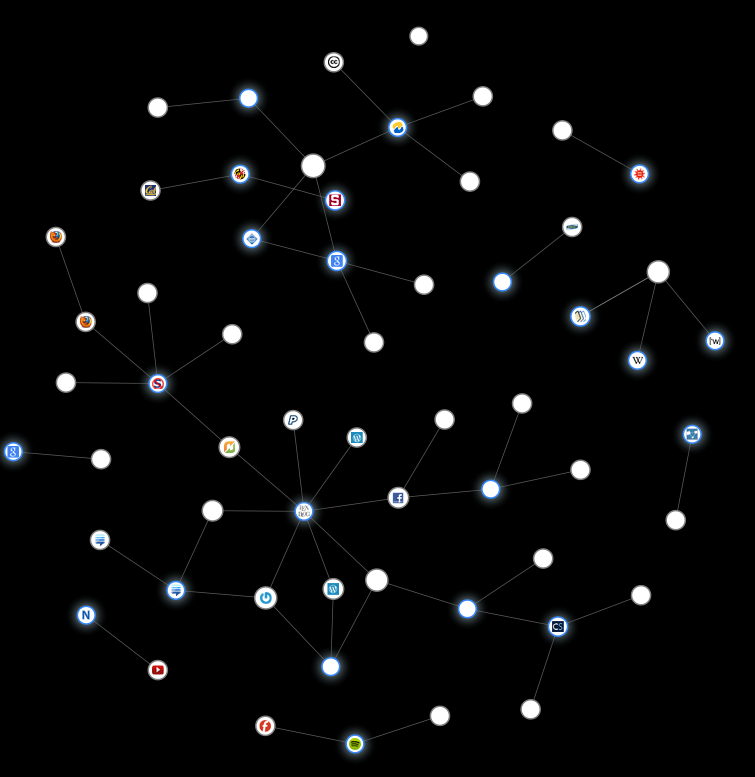
\includegraphics[height=0.7\textheight]{collusion.png}
    \caption{Skärmdump från Collusion (sedemera Lightbeam) för Firefox över 
    alla sidor som spårar mig med hjälp av denna information.}
  \end{figure}
\end{frame}


%%%%%%%%%%%%%%%%%%%%%%

\begin{frame}[allowframebreaks]{Referenser}
	\small
  \printbibliography{}
\end{frame}

\end{document}
